%%%%%%%%%%%%%%%%%%%%%%%%%%%%%%%%%%%%%%%%%%%%%%%%%%%%%%%%%%%%%%%%%%%%%%
% LaTeX Example: Project Report
%
% Source: http://www.howtotex.com
%
% Feel free to distribute this example, but please keep the referral
% to howtotex.com
% Date: March 2011 
% 
%%%%%%%%%%%%%%%%%%%%%%%%%%%%%%%%%%%%%%%%%%%%%%%%%%%%%%%%%%%%%%%%%%%%%%
% How to use writeLaTeX: 
%
% You edit the source code here on the left, and the preview on the
% right shows you the result within a few seconds.
%
% Bookmark this page and share the URL with your co-authors. They can
% edit at the same time!
%
% You can upload figures, bibliographies, custom classes and
% styles using the files menu.
%
% If you're new to LaTeX, the wikibook is a great place to start:
% http://en.wikibooks.org/wiki/LaTeX
%
%%%%%%%%%%%%%%%%%%%%%%%%%%%%%%%%%%%%%%%%%%%%%%%%%%%%%%%%%%%%%%%%%%%%%%
% Edit the title below to update the display in My Documents
%\title{Project Report}
%
%%% Preamble
\documentclass[paper=a4, fontsize=11pt]{scrartcl}
\usepackage[T1]{fontenc}
\usepackage{fourier}

\usepackage[english]{babel}															% English language/hyphenation
\usepackage[protrusion=true,expansion=true]{microtype}	
\usepackage{amsmath,amsfonts,amsthm} % Math packages
\usepackage[pdftex]{graphicx}	
\usepackage{url}
\usepackage{algorithm}
\usepackage[noend]{algorithmic}


%%% Custom sectioning
\usepackage{sectsty}
\allsectionsfont{\centering \normalfont\scshape}


%%% Custom headers/footers (fancyhdr package)
\usepackage{fancyhdr}
\pagestyle{fancyplain}
\fancyhead{}											% No page header
\fancyfoot[L]{}											% Empty 
\fancyfoot[C]{}											% Empty
\fancyfoot[R]{\thepage}									% Pagenumbering
\renewcommand{\headrulewidth}{0pt}			% Remove header underlines
\renewcommand{\footrulewidth}{0pt}				% Remove footer underlines
\setlength{\headheight}{13.6pt}


%%% Equation and float numbering
\numberwithin{equation}{section}		% Equationnumbering: section.eq#
\numberwithin{figure}{section}			% Figurenumbering: section.fig#
\numberwithin{table}{section}				% Tablenumbering: section.tab#


%%% Maketitle metadata
\newcommand{\horrule}[1]{\rule{\linewidth}{#1}} 	% Horizontal rule

\title{
		%\vspace{-1in} 	
		\usefont{OT1}{bch}{b}{n}
		\normalfont \normalsize \textsc{School of Electrical and Computer Engineering} \\ [25pt]
		\horrule{0.5pt} \\[0.4cm]
		\huge ECE 6122 Final Project Report \\
		\horrule{2pt} \\[0.5cm]
}
\author{
		\normalfont 								\normalsize
        Qiang Hu, 903014525, login: qhu35\\[-3pt]		\normalsize
        \today
}
\date{}


%%% Begin document
\begin{document}
\maketitle
\begin{abstract}
\abstractname{--}
In this project, I build a simulation platform for the relay-assisted millimeter-wave (mmWave) backhaul network using C++. This platform first model the downtown Atlanta area in a three-dimensional way based on the real building location and size information extracted from Google Earth. All the buildings are model as cubiods. A number of mmWave base stations (BSs) and relays are randomly deployed on the surfaces of these buildings. As an essential propagation feature of mmWave signals, the Blockage Effect that mmWave signal cannot penetrate through most solid obstacles (e.g., buildings) is considered in the platform. Any physical link between two wireless nodes in the network is tested to determine whether the link is blocked by any building in the environment or not. After modeling the environment, an efficient path selection algorithm, which selects a limited number of relays between pair of base station nodes to form a throughput optimal multi-hop path, is implemented. The simulation platform can take different parameters, so that different sets of simulations can be conducted to investigate the impact of parameters on the throughput performance.
\end{abstract}

\section{Introduction}

\section{Implementation Details}
\subsection{Main function}
Here I first provide an explanation on the processing flow in the main function of the program, and the detailed implementation on each module will be discussed later.
\begin{enumerate}
	\item Get current time \verb|string strTime| using \verb|chrono| as time stamp.
	\begin{itemize}
		\item As the simulation platform can accept different sets of parameters, thus, I use the time stamp at the beginning of the simulation to identify different sets of simulation results.
	\end{itemize}
	
	\item Set up simulation configuration parameters through creating a \verb|SystemParameters| object \verb|sysParams|.
	\begin{itemize}
		\item The class \verb|SystemParameters| is only used store different configuration parameters. Most of the member variables are \verb|const|.
	\end{itemize}
	
	\item Set up files addresses in use.
	\begin{itemize}
		\item There are many I/O operations in the simulation. For example, before creating the building objects, the raw data stored in file have to be read in, and after buildings are created, the building vertices will be stored in file for reference.
		\item \verb|string strDataBuildings| is the file name of building raw data;
		\item \verb|string strDataBuildingVertices| is the name of the file which stores vertices of each building generated;
		\item \verb|string dataRelayNeighbors| is the name of the file which stores the LOS connectivity information among all relay nodes in the area.
		\item \verb|string strTimeStampFile| is the name of the file which stores the time stamp of the path searching simulation corresponding to each pair of source and destination base stations. 
	\end{itemize}
	
	\item Construct all buildings in the area.
	\begin{itemize}
		\item Call \verb|getBuildingInfoFromFile()| defined in ``3DModeling.cpp" to generate all buildings in the area. In the very beginning of this function, the raw data of buildings will be read in and pharsed into appropriate types of variables.
		\item \verb|vector<Building_t> buildingSet| stores all building objects.
	\end{itemize}
	
	\item Generate candidate base station locations randomly.
	\begin{itemize}
		\item Call \verb|generateCandidateBaseStations()| defined in ``3DModeling.cpp" to randomly select buildings' top vertices as candidate base stations.
		\item \verb|std::vector<Point_t> bsSet| stores all candidate base stations.
		\item As by products, \verb|vector<Point_t> roofTopRelays| stores all candidate relays which are also buildings' top vertices. This set of relays are only used when we select the simulation parameter \verb|SystemParameters.relayType| as ``Top"; otherwise, relays on surfaces will be used.
	\end{itemize}
	
	\item Select base stations based on the grid constraint.
	\begin{itemize}
		\item Call \verb|selectBaseStationPerGrid()| defined in ``3DModeling.cpp" to select part of the base stations in \verb|bsSet| as base stations in use. Here we control that each grid can only has 1 base station in one grid whose size is controlled by parameter \verb|SystemParameters.gridSize_m|.
	\end{itemize}
	
	\item Collect all candidate relays in the area.
	\begin{itemize}
		\item Call \verb|collectAllRelays()| defined in ``3DModeling.cpp" to collect all relays on each building in the area.
		\item \verb|vector<Point_t> allRelays| stores all relays.
	\end{itemize}
	
	\item If roof top relays are in use, select roof top relays according to the grid constraint through calling \verb|selectRelayPerGrid()|, which is similar to the base station grid control mentioned before.
	
	\item Check if connectivity information exists, if not, generate connectivity information; otherwise, read existed info.
	\begin{itemize}
		\item The LOS connectivity is tested through calling function \verb|exploreConnectivity()|, in which the line segment between any pair of wireless nodes in the area are tested to determine whether it is blocked or not. If it is not blocked, these two nodes will appear as the LOS neighbor of each other respectively.
		\item To fasten the simulation, if the connectivity information has already been calculated, and stored in file, the program will just call \verb|getRelayNeighborInfoFromFile()| to read the information from file. Note that this happens only when the generated relays are not changed.
		\item \verb|vector<std::vector<int>> relayNeighborList| is used to store the index of neighbor nodes of each node. 
	\end{itemize}
	
	\item Select \verb|SystemParameters.numBSPairs| pairs of source and destination base stations, the distance between which is within the range controlled by \verb|SystemParameters.bsDistanceRange_m[2]|.
	\begin{itemize}
		\item Call function \verb|generateBaseStationPairs()| to generate \verb|vector<Point_t> bsPairs|.
	\end{itemize}
	
	\item For each pair of source and destination base stations, run the optimal path finding algorithm.
	\begin{itemize}
		\item First, read the current pair of source and destination, and call \verb|addNodeToConnectivityList()| to update the connectivity information when two base station nodes are added into the network. These two nodes will also be pushed back into \verb|vector<Point_t> allNodes| after \verb|allRelays| are pushed back.
		\item Call function \verb|findPathDecodeForward()| to find the best paths under different number of hops constaint.
	\end{itemize}
	
\end{enumerate}

\subsection{3D modeling of downtown Atlanta area}
\subsubsection{Extract the raw building information from Google Earth}
The first task of building the simulation platform is to get the information of buildings on location, size and orientation, in downtown Atlanta. I extract this information from Google Earth, where the ``3D Buildings" layer is selected and applied. To simplify the modeling, all buildings are modeled as cubiods.
\begin{figure}[!ht]
	\centering
	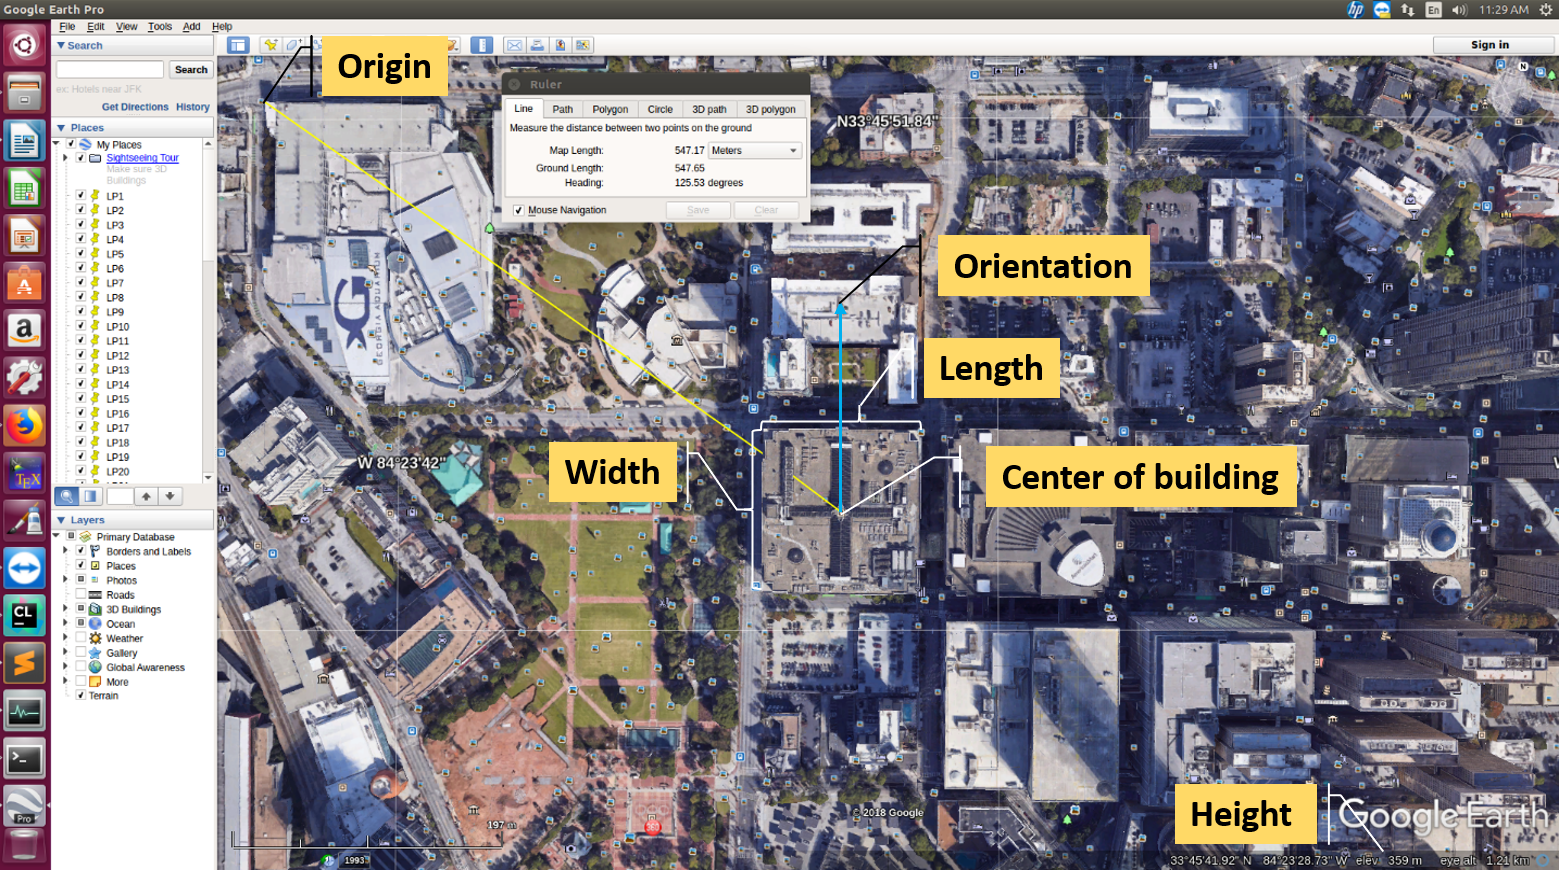
\includegraphics[width=0.95\textwidth]{./Picture2.png}
	\caption{An example of extracting the raw building information from Google Earth.}
	\label{fig: googleearth}
\end{figure}

As shown in Figure~\ref{fig: googleearth}, taking advantage of the ``ruler" tool, the distance between the center of building and the origin point can be read as r, and it is easy to calculate the 2D coordination of the center of building as $[r\sin{\theta}, r\cos{\theta}]$, where $\theta$ is the heading of the vector from origin to the building center, which is also obtained through using the ruler tool. Besides the 2D coordinates of the building center, the length, width, orientation, base level, ground level, and height of the building are also read in Google Earth. As for a single building, the raw information is organized in the following format:
\begin{table}[!ht]
	\centering
	\begin{tabular}{|c|c|c|c|c|c|c|}
		\hline
		Center.x & Center.y  & Length & Width & Height & Base & Orientation \\
		\hline
	\end{tabular}
	\caption{The format used to store raw data of buildings.}
	\label{tab:format}
\end{table}

\subsubsection{Elementary classes: Point\_t, Vector\_t, Line\_t, Plane\_t, and Building\_t}
Before reading the raw data into our C++ simulation program, a class modeling an individual building (i.e., class \verb|Building_t|) has to be defined in advance so that the read-in data can be used to initialize different building instances (objects). However, the definition of class \verb|Building_t| is further based on the definition of class \verb|Point_t|, because all the vertex points of a cubiod (i.e., building) and the randomly deployed candidate relay locations are stored in a \verb|Building_t| object as member variables in type \verb|Point_t|. To implement the class \verb|Point_t|, class \verb|Vector_t| which defines the properties and operations of a space vector is introduced. Actually, class \verb|Point_t| and class \verb|Vector_t| use each other in both definitions. Based on class \verb|Point_t| and class \verb|Vector_t|, a new class \verb|Line_t| is defined to capture the features of a line segment in the space. Furthermore, as there are six faces of a cubiod, I create a new class \verb|Plane_t| to describe the characteristics of each face of a cubiod in the space.  

\begin{itemize}
	\item \textbf{Class} \verb|Point_t|:
\end{itemize}

Thus, here I first give a brief introduction on class \verb|Point_t|. It has four private member variables: \verb|double x, y, z;| and \verb|bool valid|. \verb|x, y, z| are used to store the coordination of a point, while \verb|valid| is used to identify whether this point object is a valid point or not, as in some cases the program has to return a ``NULL" point object whose \verb|valid| equals \verb|false|. 

Three constructors are provided to accept different argument types. 

Several utility methods are also defined as member methods in \verb|Point_t|, for example, \verb|distanceTo()| returns the distance between \verb|*this| to another point. It is noticed that three utility methods use the definition of another class \verb|Vector_t|, and they are \verb|destinationTo()|, \verb|sourceFrom()|, and \verb|vectorTo()|. The detailed explanation of these methods can be found in the comments in ``./Point\_t.h". Moreover, a method named \verb|sameAs()| is defined to compare the value between \verb|*this| and another point.

\begin{itemize}
	\item \textbf{Class} \verb|Vector_t|:
\end{itemize}

In the \verb|Vector_t| class, three private member variables \verb|double x, y, z| are used to store the coordinates of a space vector in a euclidean coordinate system. Six constructors are defined to fit different input arguments.

As in class \verb|Point_t|, the operations of a vector such as ``mod", ``plus", ``minus", ``times", ``divide", ``dot product", and ``cross product" are also defined in this class.

\begin{itemize}
	\item \textbf{Class} \verb|Line_t|:
\end{itemize}

Member variables \verb|Point_t src, dst| defines the two end points of a line segment. \verb|Vector_t sd| is the vector from \verb|src| to \verb|dst|, and \verb|Vector_t dir| is the normalized version of \verb|sd|, which only contains the direction information of this vector. Only one constructor is defined. 

This class is mainly used in the blockage test where a line segment is tested whether it intersect with any face of any building in the area. 

\begin{itemize}
	\item \textbf{Class} \verb|Plane_t|:
\end{itemize}

As mentioned above, all buildings are modeled as cubiods, thus all faces are rectangles, so that four \verb|Point_t| member variables \verb|v1, v2, v3, v4| are defined to store the four vertices of a face. Additionally, the \verb|normal| vector of the plane is also defined as a member variable. Two constructors are defined, one of which is used when we initialize a face using four \verb|Point_t| objects; while the other is used when the plane is defined by a normal \verb|Vector_t| and a \verb|Point_t|.

The key part in \verb|Plane_t| is to define the methods of testing the intersection relationship between a line segment and a face. Member method \verb|planeIntersectLine()| receives \verb|Line_t l| as argument, and return a \verb|Point_t| which is the intersection point of \verb|Line_t l| and \verb|*this| plane. It is noticed that, if the line segment and the face has no intersection point, the returned \verb|Point_t| variable's \verb|valid| property is set as \verb|false|. 

The general idea of the test is that the program firstly test that whether the line segment is parallel to the plane. If they are parallel, they do not intersect. Noticed that it is assumed that if the line segment is in the plane, it is considered not intersected. If they are not parallel to each other, it means there is one intersection point between the line and the plane. The algorithm utilizes the geometric knowledge to calculate the coordinate of the intersection point. After that, two more steps are conducted to test whether the intersection point is within the line segment and whether the intersection point is within the rectangle face. If both cases are \verb|true|, the calculated intersection point will be returned; otherwise, no intersection exists.

\begin{itemize}
	\item \textbf{Class} \verb|Building_t|:
\end{itemize}

The \verb|Building_t| class stores the raw data information of this building in its member variables, and it also stores the vertices of the cubiod modeled as well. Besides, as mentioned in the introduction section, the candidate relay locations are randomly deployed on the surfaces of the building except the bottom face. \verb|vector<Point_t> Relays| are defined to store all relay \verb|Point_t| on the building. As the base stations are also deployed on the buildings in the area, if one base station is on this building, its member variable \verb|bool hasBS| is set as \verb|true|.

When the constructor is called, several member methods are called to complete the initialization of the \verb|Building_t| object. \verb|VertexGenerator()| is used to generate the different vertices of the cubiod using the center point coordinates, length, height, and orientation information. \verb|RelayGenerator()| is called to randomly generate candidate relay locations on the surfaces, and the density is pre-set in the \verb|SystemParameter| object \verb|sysParam|. The generation of the relays are done face by face, thus a function \verb|GenerateRelayOnFace()| is defined. After the relays on each face are generated, \verb|RelayGenerator()| collects all relays together and store them in \verb|vector<Point_t> Relays|.\\

With all above classes defined, the 3-D modeling part is completed, and now we shall move on to see how the blockage test is handled.

\subsection{Blockage test}
The blockage test is essential in this simulation platform, because in my research, only LoS paths will be used to establish mmWave links. If a path between a pair of nodes are blocked by a building, no mmWave link will be considered to establish between them. To implement the blockage test, I define a method \verb|blockageTest()| in the ``./3DModeling.cpp" file.

In \verb|blockageTest()|, a line segment is tested whether it is intersected with any building in the area. The pseudo code of the alogrithm is shown as follow.
\begin{algorithm}[!ht]
	\caption{Blockage test}
	{\fontsize{10}{10}\selectfont
		\begin{algorithmic}[1]
			\renewcommand{\algorithmicrequire}{\textbf{Input:}}
			\renewcommand{\algorithmicensure}{\textbf{Output:}}
			\REQUIRE $sd$, $buildingSet$
			\ENSURE  $blocked$
			\STATE $blocked \leftarrow$ false;
			\FOR {$bldg$ in $buildingSet$}
			\STATE $sIsTopV \leftarrow$ false; $dIsTopV\leftarrow$ false;
			\STATE $faceIntersectCount \leftarrow$ 0; $sdOnEdgeCount \leftarrow$ 0;
			\IF {$sd.src$ == any top vertex of $bldg$}
			\STATE $sIsTopV \leftarrow$ true;
			\ENDIF
			\IF {$sd.dst$ == any top vertex of $bldg$}
			\STATE $dIsTopV \leftarrow$ true;
			\ENDIF
			\FOR {$face$ in $bldg$'s faces}
			\STATE $testIntP \leftarrow$ face.planeIntersectLine(sd);
			\IF {$testIntP.valid$}
			\IF {$testIntP$ != $sd.s$ \&\& $testIntP$ != $sd.d$}
			\RETURN true;
			\ELSE
			\STATE $faceIntersectCount++$;
			\IF {$face$ is side face or top face}
			\IF {$sd.src$ or $sd.dst$ is on any $face$'s edge}
			\STATE $sdOnEdgeCount++$;
			\ENDIF
			\ENDIF
			\ENDIF
			\ENDIF
			\ENDFOR
			\IF {$faceIntersectCount$ >= 5}
			\RETURN true;
			\ENDIF
			\IF {$faceIntersectCount$ == 4 || $faceIntersectCount$ == 3}
			\IF {!($sIsTopV$ \&\& $dIsTopV$)}
			\RETURN true;
			\ENDIF
			\ENDIF
			\IF {$faceIntersectCount$ == 2}
			\IF {!($sIsTopV$ \&\& $dIsTopV$)}
			\IF {$sdOnEdgeCount == 0$}
			\RETURN true;
			\ENDIF
			\ENDIF
			\ENDIF
			\ENDFOR
			\RETURN blocked;
		\end{algorithmic}
		}
\end{algorithm}

Here I do not provide detail explanation on the algorithm, details can be found in the comments in the source code. But the general idea is to count the total number of intersection points between the line segment and the building, and determine the intersection status based on the count. Note that, the line segment has intersect point to the building does not mean it is always the case a blockage happens. In fact, any line segment in the simulation must starts from a certain base station or relay node, which is exactly on the building, and it means a line segment must always intersect with at least one building and there at least exists one intersection point; however, as long as this line segment is not blocked, the \verb|blockageTest()| function returns \verb|false|.

\subsection{Optimal path searching algorithm}
The optimal searching algorithm is describe as shown in the following pseudo code.

\begin{algorithm}[h!]
	\caption{Finding the path with maximum throughput}
	{\fontsize{10}{10}\selectfont
		\begin{algorithmic}[1]
			\renewcommand{\algorithmicrequire}{\textbf{Input:}}
			\renewcommand{\algorithmicensure}{\textbf{Output:}}
			\REQUIRE $src$, $dst$, $relays$, $numHop$, $bW$
			\ENSURE  $maxPath$
			% \\ \textit{Initialisation} :
			\STATE $nodes.\mathrm{add}(relays,src,dst)$; // $nodes$ stores all nodes
			\FOR {$node$ in $nodes$} 
			\STATE $iNbs.\mathrm{add}(\mathrm{findAllLoSNbs(node,nodes)})$;
			\STATE $iNbsList.\mathrm{add}(iNbs)$; // store indices of neighbors
			\ENDFOR
			\STATE Initialize $allPaths$ as an empty list of paths;
			\STATE $minSL = $ Inf; // minimum schedule length;
			\FOR {$maxHop = 1:numHop$}
			\STATE Initialize $path$ as an empty list of nodes' indices;
			\STATE $path.\mathrm{add}(iSrc)$; // $iSrc$ is the index of $src$ in $nodes$ 
			\STATE $iHop = 1$; // the index of current hop;
			\STATE $\mathrm{searchNextNode}(path,iHop,maxHop)$;
			\ENDFOR
			\STATE $maxPath = allPaths.\mathrm{get}(end)$;
			\\ \textit{Function}: void $\mathrm{searchNextNode}(path,iHop,maxHop)$
			\IF {$iHop \leq maxHop$}
			\STATE $iPreNode = path.get(iHop-1)$;
			\STATE $iCurNbs = iNbsList.get(iPreNode)$;
			\FOR {$iNb$ in $iCurNbs$}
			\STATE Calculate the sum of demand of the current link and the previous
			link as $sumDemand$.
			\IF {($sumDemand \geq minSL$)}
			\RETURN
			\ENDIF
			% \IF {($lMin \leq lCurLink \leq lMax$)}
			\IF {($!\mathrm{intfTest}(iNb,path,iHop,bW)$)}
			\STATE $path.\mathrm{add}(iNb)$;
			\IF {($nodes.get(iNb) == dst$)}
			\STATE $allPaths.\mathrm{add}(path)$;
			\STATE $minSL = \mathrm{calMinSL}(path,iHop)$;
			\ENDIF
			\IF {($nodes.get(iNb) != dst$)}
			\STATE $\mathrm{searchNextRelay}(path,iHop+1,maxHop)$;
			\ENDIF
			\ENDIF
			% \ENDIF
			\ENDFOR
			\ENDIF
			\RETURN maxPath;
		\end{algorithmic}
	}
\end{algorithm}
First, only the LoS neighbors of each $node$ (Lines 2--4) are considered as 
candidate nodes to be selected in one step.  The start of a path is the 
given source node (Line 9).  The main loop of the algorithm does a
\textit{depth-first} search for a maximum throughput path using a progressively 
larger maximum number of hops, $maxHop$, at each iteration (Lines 7--11).  The 
paths found at one iteration help bound the search done at the next iteration.

In the depth-first search (Line 13--27), when the index of current hop does not 
exceed $maxHop$ (Line 13), the selection of a candidate node makes the current 
path invalid in the following cases: (1) the sum of link demand of the current 
link (i.e., from the previous node to the selected node) and the previous link in 
the path exceeds the current minimum schedule length (Lines 18--19); (2) the  
candidate node will be interfered by previously selected nodes in the path (Line 
20). If neither of the above cases occurs, the node is added to the current path 
(Line 21).  If the selected node is the destination, the path is added to the 
path list and the minimum schedule length is updated (Lines 22--24).  Otherwise, 
the search continues to the next hop (Line 25--26).  At the end, the last path
added to the list is the maximum throughput path. Note that condition (1) is from 
Theorem in my paper, and the minimum schedule length value is propagated 
from one iteration of the main loop to the next and this helps eliminate many 
possible paths in performing the depth-first search to a given maximum number of 
hops.

The time complexity of Algorithm 1 is $O(D^M)$, where $D$ is the maximum degree
of the connectivity graph of candidate relay locations and $M$ is the maximum
hop count for a path.  Two relay locations are neighbors in the connectivity
graph if they have a LoS path between them.  In the worst case, the time 
complexity is $O(N^M)$, where $N$ is the total number of candidate relay
locations but, due to the large number of obstacles in urban areas,
$D\ll N$, typically.

\end{document}